\documentclass[a4paper, 12pt]{article}

\usepackage{fancyhdr}
\usepackage[top=0.5in,bottom=0.5in,left=0.5in,right=0.5in]{geometry}
\usepackage{graphicx}
\usepackage{empheq}
\usepackage{ifthen}
\usepackage{cases}
\usepackage{epstopdf}
\usepackage{listings}
\usepackage{amsmath}
\usepackage{amssymb}
\usepackage{enumerate}
\usepackage[miktex]{gnuplottex}
\usepackage{gensymb}
\usepackage{tikz}
\usepackage{float}
\usepackage{subcaption}
\usepackage{enumitem}
\usepackage{textcomp}
\usepackage[utf8]{inputenc}
\usepackage[english]{babel}
\usetikzlibrary{shapes,arrows,positioning,shadows,calc}

\usepackage{color}
\definecolor{orange}{rgb}{1,0.5,0}
\definecolor{lightgray}{rgb}{.9,.9,.9}
\definecolor{xml_keyword}{rgb}{0.37, 0.08, 0.25}
\definecolor{xml_string}{rgb}{0.06, 0.10, 0.98}
\definecolor{xml_comment}{rgb}{0.12, 0.38, 0.18}
\definecolor{xml_doc}{rgb}{0.25,0.35,0.75}

\newcommand{\norm}[1]{\left\lVert#1\right\rVert}

\graphicspath{{./images/}}


\title{\textbf{Introduction to Neuroinformatics} \\Summary of the lectures
2018\\\normalsize Version 4.0 \\
for internal use by students attending the lecture only}

\author{
\texttt{Initial Version 2012}\\
	Benjamin Ellenberger
\and
\texttt{Revision 2013}\\
	Joachim Ott\\Dora Sumislawska
\and
\texttt{Revision 2014}\\
	Fabian Tschopp
\and
\texttt{Revision 2018}\\
	Vanessa Leite}

\date{}


\begin{document}
\maketitle
\newpage
\tableofcontents
\newpage

\section{Neuroinformatics}
\subsection{Introduction}
\begin{itemize}[noitemsep,nolistsep]
	\item Human brain on average: $1.5 kg$ weight, $1.2 l$ volume.
	\item Human brains are large, but by far not the largest (for instance, elephants and whales have bigger brains).
	\item The brain mainly is there to receive stimuli from the environment, encode it, do sensory integration and finally decode to make movements, actions and decisions.
	\item The cells (neurons) that make up brains are very similar between species.
	\item Some neuron types occur in specific parts of the brain and it is consistent between species.
	\item A neuron is a processing unit that receives electrical input and generates electrical output.

\end{itemize}
\begin{figure}[htbp]
	\centering
	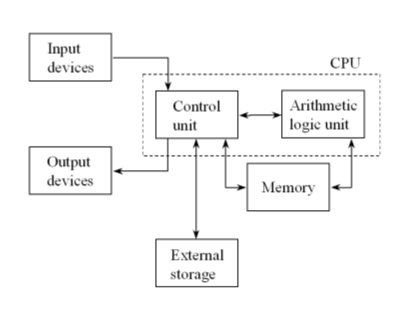
\includegraphics[scale=0.6]{1_2.jpg}
 	\caption{Turing Machine / CPU}
\end{figure} 

\paragraph{How information is processed in the brain?}
We can consider many levels when we talk about the brain processing information. From the highest to the lowest level: behavior $\rightarrow$ system and pathways $\rightarrow$ circuits $\rightarrow$ neurons $\rightarrow$ microcircuits $\rightarrow$ synapses $\rightarrow$ membrane potential (molecules and ions). \\

\textbf{Differences between a brain and a computer (what the brains have):}
\begin{itemize}[noitemsep,nolistsep]
	\item Massive parallelism
	\item Constantly adapting
	\item Chemical signaling
	\item Unreliable units (brain is noisy compared to a computer)
	\item Analog computation
	\item Robust to damage
	\item Very energy efficient
	\item Memory fixed in place (as part of each processing unit).
\end{itemize}
\textbf{Similarities between a brain and a computer:}
\begin{itemize}[noitemsep,nolistsep]
	\item Process information
	\item Logical operations
	\item Memory
	\item Use electrical (digital) signaling
	\item Can learn from inputs
	\item Consume energy
\end{itemize}

\paragraph{Easy vs Dificult tasks}
Things that we can do and computer can't, change over time. Things that are easy to humans can be hard to a computer, mostly because we don't know how to simulate a brain. We do things without think consciously about it.

\begin{itemize}
\item It is comparatively easy to make computers exhibit adult level performance on intelligence tests or playing checkers, and difficult or impossible to give them the skills of a one-year-old when it comes to perception and mobility.” – Hans Moravec
\end{itemize}

\paragraph{Neurons structure}
\begin{itemize}[noitemsep,nolistsep]
	\item Membrane: Separates inside from outside.
	\item Soma: Cell body, contains nucleus and organelles.
	\item Dendrites: Connect to soma, provide inputs to soma.
	\item Axons: Connects to soma, conducts away from soma. Often myelinated and ends in synapses. Carries output.
	\item Synapse: Pre- and postsynaptic terminals, transmit information between neurons.
	\item In the order of magnitude, there are about 10'000 synapses per neuron.
\end{itemize}

\textbf{Other facts}
\begin{itemize}[noitemsep,nolistsep]
	\item An 83000-Processor supercomputer can only match $1\%$ of the human brain.
	\item C. Elegans (worm) has 302 nerve cells, a frog 16M, a cat 1B and a human 85B.
	\item Human brain project aims to simulate the entire human brain on computers.
	\item More efficient simulations of brain behavior by Neurogrid or IBM TrueNorth.
	\item Number of neurons in human brain: $\sim10^{11}$, synapses: $\sim10^{15}$.
	\item Number of genes in human genome: $\sim$25000.
	\item WindowsXP contains more code (1.5Gb) for operating a personal computer than DNA ($\sim$750Mb) to generate life.
	\item Deep Neural Networks were inspired by the brain in the beggining but it is not like the brain (neurons) works.
	
\end{itemize}

\section{Nervous System Organization}
\subsection{Anatomy}
\begin{itemize}[noitemsep,nolistsep]
	\item Central nervous system (CNS): Brain and spinal cord.
	\item Peripheral nervous system (PNS): Somatic, autonomic (sympathetic and parasympathetic) NS.
	\item Brain cuts: Horizontal plane cut, coronal/frontal cut and sagittal cut (between eyes). Cross-section through spinal cord, for example.
	\item The skull protects, meninges envelope the CNS and has 3 layers, the dura mater, arachnoid mater and pia mater. Primary function is protection.
	\item The cortex is the layer directly under the surface of the brain.
	\item There are 4 lobes in each hemisphere. Lobes are separated by fissures in the cortex.
\end{itemize}
\begin{figure}[H]
	\centering
	\begin{subfigure}[b]{0.5\textwidth}
		\centering
		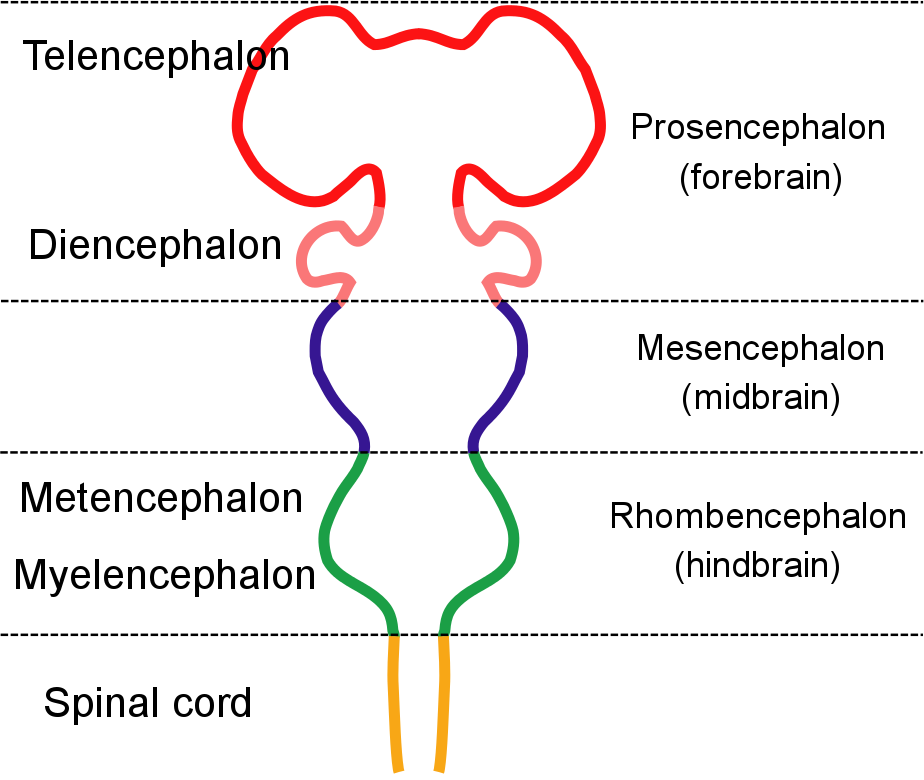
\includegraphics[width=\textwidth]{brain-parts.png}
	\end{subfigure}%
	~
	\begin{subfigure}[b]{0.5\textwidth}
		\centering
		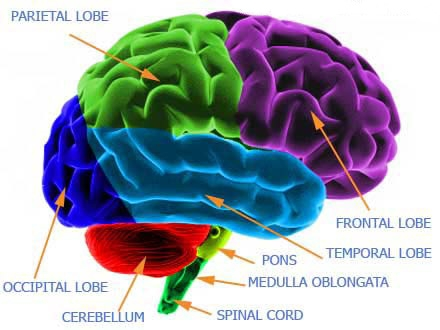
\includegraphics[width=\textwidth]{brain.png}
	\end{subfigure}
\end{figure}
\begin{figure}[H]
	\centering
	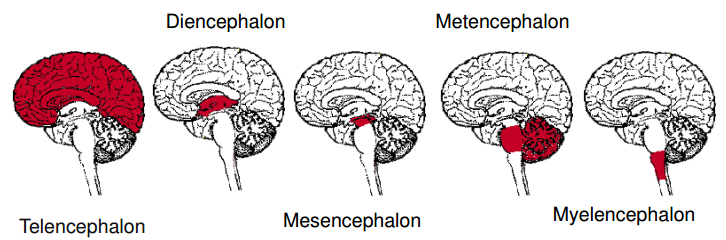
\includegraphics[width=\textwidth]{brain_anatomy_01.png}
\end{figure}
\begin{figure}[H]
	\centering
	\begin{subfigure}[b]{0.5\textwidth}
		\centering
		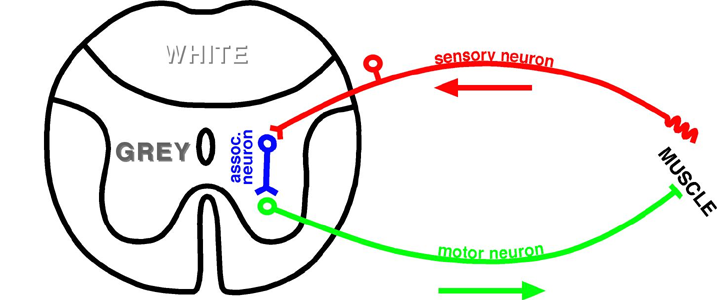
\includegraphics[width=\textwidth]{motor-sensory-neuron.png}
	\end{subfigure}%
	~
	\begin{subfigure}[b]{0.5\textwidth}
		\centering
		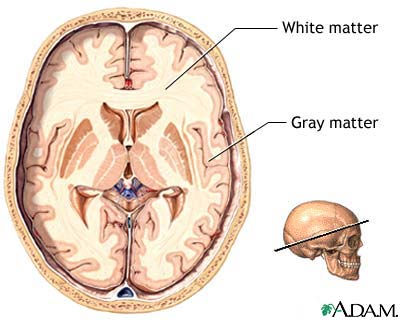
\includegraphics[width=\textwidth]{brain-cut.png}
	\end{subfigure}
\end{figure}

\subsection{Building elements of the brain}
\begin{itemize}[noitemsep,nolistsep]
	\item Forebrain (Prosencephalon): Cortex, thalamus, hippocampus, basal ganglia, corpus callosum.
	\item Midbrain (Mesencephalon): Tectum, tegmentum.
	\item Hindbrain (Rhombencephalon): Cerebellum, pons, medulla oblongata.
	\item White matter: Glia cells, myelinated axons.
	\item Grey matter: Neurons (soma).
	\item Neocortex: Six-layered cortex that forms the surface of most of the cerebral hemispheres.
	\item Corpus callosum: Midline fiber bundle, connects the two cerebral hemispheres.
	\item Gyrus: Ridges of the cotex, with valleys (sulci).
\end{itemize}
\subsubsection{The limbic system}
\begin{itemize}[noitemsep,nolistsep]
	\item Structure: On medial and basal surfaces of cerebral hemispheres.
	\item Includes cingulate gyrus, parahippocampal gyrus, hippocampal formation, fornix, amygdala, septum, mamillary bodies
	\item Function: Emotional expression, memory acquisition, fear conditioning, violence and aggression.
\end{itemize}
\begin{figure}[H]
	\centering
	\begin{subfigure}[b]{0.5\textwidth}
		\centering
		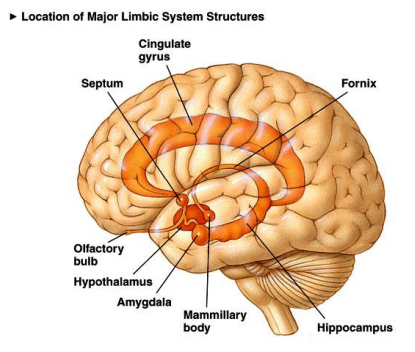
\includegraphics[width=\textwidth]{brain_anatomy_02.png}
	\end{subfigure}%
	~
	\begin{subfigure}[b]{0.5\textwidth}
		\centering
		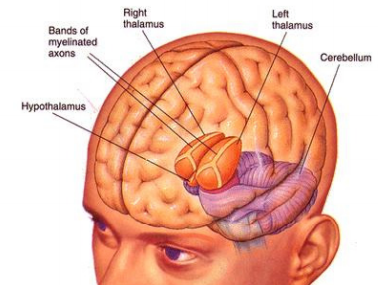
\includegraphics[width=\textwidth]{brain_anatomy_03.png}
	\end{subfigure}
\end{figure}
\subsubsection{Hypothalamus and thalamus}
\begin{itemize}[noitemsep,nolistsep]
	\item Structure: Relatively large, two symmetric large nuclei, many projections.
	\item Function: Relay station, domain-specific information processing.
	\item The upper brain stem is the diencephalon.
	\item The hypothalamus is very small and controls autonomic mechanisms.
\end{itemize}
\subsubsection{Basal ganglia}
\begin{itemize}[noitemsep,nolistsep]
	\item Structure: Collection of nuclei embedded deep within the cortex.
	\item Partially surrounds the thalamus.
	\item Sensory projectons to the cerebrum
	\item Function: Regulate voluntary movement.
	\item Movement disorders like Parkinson's.
\end{itemize}
\subsubsection{Cerebellum}
\begin{itemize}[noitemsep,nolistsep]
	\item Structure: ``little brain'', has layered appearance and symmetry.
	\item Two hemispheres are connected by the vermis.
	\item Function: Coordinated motor behavior, posture adjustments and stores memories for simple learned motor responses.
\end{itemize}
\subsubsection{Reticular Formation}
\begin{itemize}[noitemsep,nolistsep]
	\item Structure: Diffuse arrangement of ascending and descending neurons.
	\item Function: Arousal, selective attention, respiration.
\end{itemize}
\subsubsection{Connections}
\begin{itemize}[noitemsep,nolistsep]
	\item The Basal ganglia projects to the cerebral cortex (via thalamus).
	\item The cerebellum projects to the cerebral cortex (via thalamus).
	\item The cerebral cortex projects to basal ganglia, cerebellum and motor neurons (and interneurons) via  pons.
\end{itemize}
\begin{figure}[H]
	\centering
	\begin{subfigure}[b]{0.5\textwidth}
		\centering
		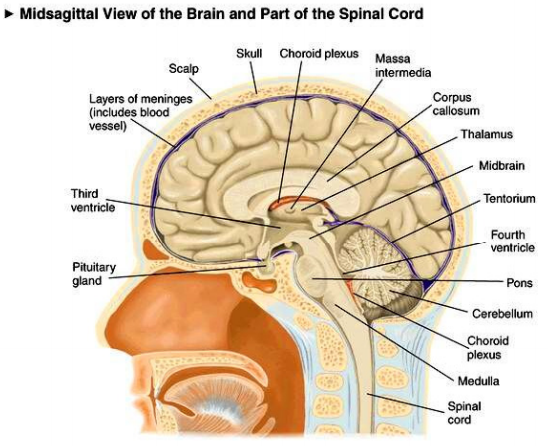
\includegraphics[width=\textwidth]{brain_anatomy_04.png}
	\end{subfigure}%
	~
	\begin{subfigure}[b]{0.5\textwidth}
		\centering
		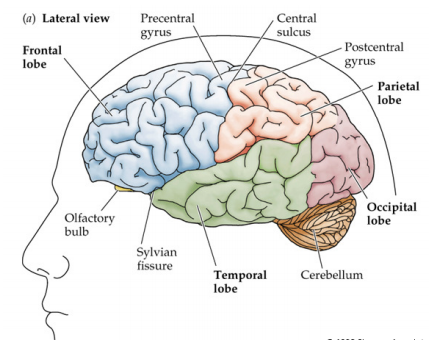
\includegraphics[width=\textwidth]{brain_anatomy_05.png}
	\end{subfigure}
\end{figure}

\subsection{Nervous system in numbers}
\begin{itemize}[noitemsep,nolistsep]
	\item $1\,mm^3$ of white matter is $9\,m$ of axons.
	\item $1\,mm^3$ of grey matter is $50'000$ neurons.
	\item In $1\,mm^3$ about $100'000$ cells.
	\item The cortex has six layers.
\end{itemize}

\subsection{Basic structure of the neuron}
\subsubsection{Components}
\begin{itemize}[noitemsep,nolistsep]
	\item Cell body
	\item Nucleus
	\item Dendrite: Input component.
	\item Axon: Output component, makes contact to other neurons.
	\item Myelin: Wraps around axons, makes white matter white.
	\item Boutons: At the ends of the axons, connects neurons.
	\item Soma: Body of a cell without it's extensions.
	\item Afferent: Neurons that carry nerve impulses from receptors to the CNS.
	\item Efferent: Neurons that carry information away from the CNS.
	\item Projection neuron: Neuron with long axons that project to distant targets.
\end{itemize}
\subsubsection{Axon transport}
\begin{itemize}[noitemsep,nolistsep]
	\item Golgi apparatus sits at the cell body.
	\item Transport of vesicles to the axon terminal (anterograde).
	\item Transport of empty vesicles back to the cell body (retrograde).
\end{itemize}
\subsubsection{Synapse}
\begin{itemize}[noitemsep,nolistsep]
	\item Boutons: connection point.
	\item Cleft: Little gap between presynaptic and postsynaptic neuron.
	\item Dendritic spines: Dendritic part of the synapse.
	\item Transmitter: Gets released by the presynaptic neuron, in vesicles.
	\item Vesicles: Transport the transmitter inside the cell.
	\item Receptors: Binding site for the transmitter.
\end{itemize}

\subsection{Muscle reflex and antagonistis}
\subsubsection{Reciprocal innervation of antagonistic muscles}
\begin{enumerate}[noitemsep,nolistsep]
	\item A tack produces a burst of firing (sensory neurons, for example on the finger).
	\item The burst excites excitatory spinal interneurons, which then excite the motor neurons of a muscle.
	\item The burst also excites inhibitory spinal interneurons that inhibit antagonist muscle motor neurons.
	\item One muscle gets contracted, the other relaxed, allowing for a rapid flexion. No brain involved (but gets informed).
\end{enumerate}
\subsubsection{Elicitation of a stretch reflex}
\begin{itemize}[noitemsep,nolistsep]
	\item When hitting the knee tendon with a hammer, the spindles of the thigh muscle get stretched and this elicits a burst of firing in the spindle afferents.
	\item The burst triggers a burst of firing in the thigh muscle motor neurons, causing contraction.
\end{itemize}

\section{Membrane Potential}
\subsection{Introduction}
In the lowest level, the brain process information in each processing unit (neurons) through membrane potential, molecules and ions.

Experiments in visual area of monkeys and cats (V1 recordings) allowed us to know more about the visual system. We now know that the visual system has orientation selectivity and the MT area respond to motion/velocity.

\href{https://www.youtube.com/watch?v=8VdFf3egwfg}{Here} you can see an experiment and hear the neurons firing.

\subsection{Membrane structure}
\begin{itemize}[noitemsep,nolistsep]
	\item The membrane is bilayer and creates an energy barrier.
	\item Ions can not just flow through. Channels and pumps are needed.
	\item ECS: Extra cellular solution.
	\item ICS: Intra cellular solution.
	\item Membrane is built of two types of molecules, charged hydrophilic dipole head-group (outside) and an uncharged, hydrophobic hydrocarbon tail.
	\item It is a phospholipid bilayer.
\end{itemize}

\subsection{Hyperpolarization}
\begin{itemize}[noitemsep,nolistsep]
	\item The extracellular space has potential $V=0\,mV$.
	\item The intracellular space has resting potential $V=-70\,mV$.
\end{itemize}

\subsection{Inputs to neurons, excitatory}
\begin{itemize}[noitemsep,nolistsep]
	\item Inputs to neurons over synapses.
	\item Depolarization, about $V=30\,mV$ presynaptic.
	\item Excitatory current is positive charge, which comes from the extra- to intra-cellular space.
	\item The signal is analog and graded.
	\item On the way to the soma, the intra-cellular current gets reduced by leak current (positive charge) that leaves the intra-cellular space.
	\item From the large depolarization ($V=0\,mV$), about $V=-69.5\,mV$ is the value at the soma.
	\item EPSP (excitatory postsynaptic potential) $0.2$ to $0.4\,mV$.
	\item Spatial and temporal spread of the signal.
	\item $\tau_m$ defines how fast potentials changes.
	\item $\lambda$ defines how far currents travel.
\end{itemize}
\begin{figure}[H]
	\centering
	\scalebox{0.7}{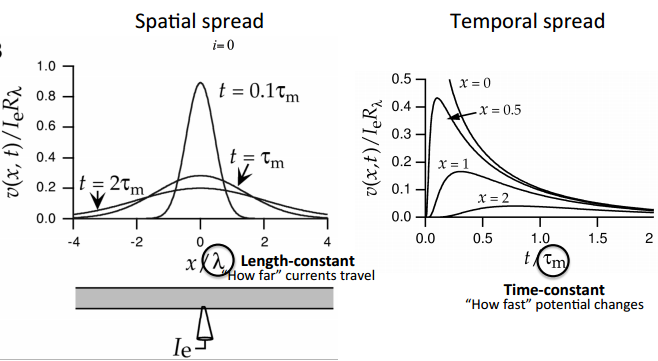
\includegraphics{spatial_temporal_spread.png}}
\end{figure}

\subsection{Chemical synapses}
\begin{figure}[H]
	\centering
	\scalebox{0.7}{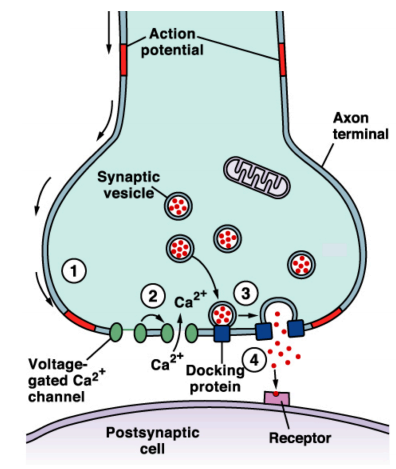
\includegraphics{chemical_synapse.png}}
\end{figure}
\begin{itemize}[noitemsep,nolistsep]
	\item Digital transmission, but can have failures, and graded release.
	\item There can even be synapses directly on the soma or axon.
\end{itemize}

\subsection{Inhibitory post-synaptic potential}
\begin{itemize}[noitemsep,nolistsep]
	\item Depolarization, about $V=30\,mV$ presynaptic.
	\item A large hyperpolarization, $V=-90\,mV$ at postsynaptic dendrite.
	\item Small hyperpolarization at soma, $V=-70.2\,mV$.
\end{itemize}

\subsection{Summation of Inputs}
\begin{itemize}[noitemsep,nolistsep]
	\item Temporal summation, one input after another.
	\item Spatial summation, inputs from different dendrite branches.
	\item Summing up, the threshold is crossed.
	\item Typically 20 to 30 Inputs are needed to go above threshold.
	\item The action potential gets triggered at the beginning of the axon.
	\item The threshold is about $-60\,mV$.
\end{itemize}

\subsection{Action potential}
\begin{itemize}[noitemsep,nolistsep]
	\item Has an active regenerative process.
	\item The duration is about 1 to 2 ms.
	\item All-or-none (digital).
	\item Amplitude gets converted into rate.
	\item Components: Depolarization, overshoot ($>0\,mV$), repolarization/hyperpolarization and a refractory period (back to $-70\,mV$).
	\item Peak about $0.5\,ms$ long, $4.4\,ms$ refractory period.
\end{itemize}
\begin{figure}[H]
	\centering
	\begin{subfigure}[b]{0.5\textwidth}
		\centering
		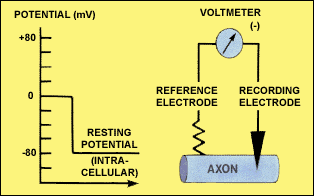
\includegraphics[width=\textwidth]{voltage-source-in-membrane.png}
	\end{subfigure}%
	~
	\begin{subfigure}[b]{0.5\textwidth}
		\centering
		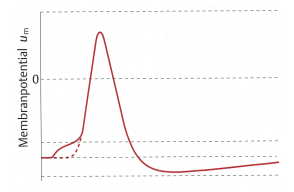
\includegraphics[width=\textwidth]{action_potential_01.png}
	\end{subfigure}
\end{figure}
\begin{figure}[H]
	\centering
	\begin{subfigure}[b]{0.5\textwidth}
		\centering
		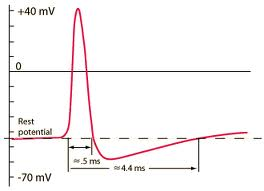
\includegraphics[width=\textwidth]{voltage-source-in-membrane2.png}
	\end{subfigure}%
	~
	\begin{subfigure}[b]{0.5\textwidth}
		\centering
		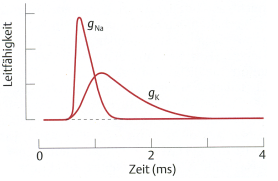
\includegraphics[width=\textwidth]{action_potential_02.png}
	\end{subfigure}
\end{figure}

\subsection{Axon}
\begin{itemize}[noitemsep,nolistsep]
	\item Myelin sheet is often wrapped around the axon.
	\item This makes the white-matter white.
	\item Myelin is an electrical insulator which grants faster propagation.
	\item Less energy is needed with myelinated axons.
	\item The current goes through the node of ranvier (myelin sheath gaps).
\end{itemize}

\subsection{Ionic currents and equilibrium}
\subsubsection{Receptors:}
\begin{itemize}[noitemsep,nolistsep]
	\item Excitatory: AMPA/NDMA, mixed cation, $V(drive) =0\,mV$
	\item Inhibitory: GABA A, chloride (Cl), $V(drive) =-65\,mV$
	\item Inhibitory: GABA B, potassium (K), $V(drive) =-90\,mV$
\end{itemize}
\subsubsection{Action potential:}
\begin{itemize}[noitemsep,nolistsep]
	\item Sodium (Na): $V(drive) = 55\,mV$
	\item Potassium (K); $V(drive) = -90\,mV$
\end{itemize}

\subsubsection{Ion equilibrium}
\textbf{Charge carrier (giant squid axon)}:\\
\begin{tabular}{|l|l|l|l|}
	\hline
	Ion type & Cytoplasm (mM) & Extracellular (mM) & Equilibrium potential (mV)\\\hline
	$K^+$ & 400 & 20 & -75 \\\hline
	$Na^+$ & 50 & 440 & +55\\\hline
	$Cl^-$ & 52 & 560 & -60\\\hline
	$Ca^{2+}$ & 0.0001 & 10 &\\\hline
	Organic anions & 385 & - &\\\hline
\end{tabular}
\begin{figure}[H]
	\centering
	\scalebox{0.5}{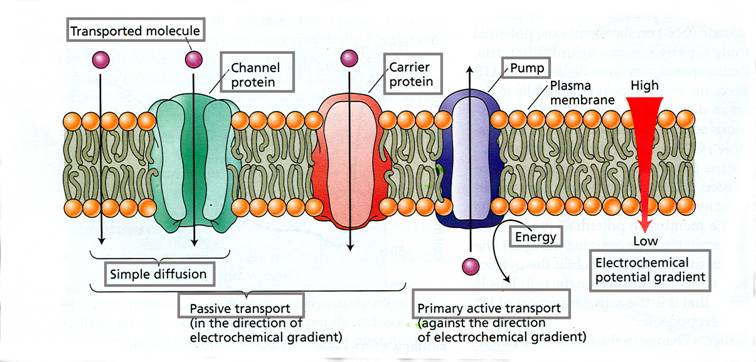
\includegraphics{bilayer-closeup2.png}}
\end{figure}

\subsection{Nernst-Equation}
\subsubsection{Acting forces}
\begin{itemize}[noitemsep,nolistsep]
	\item Ion concentration gradient (diffusion).
	\item Electric potential (electrostatic force).
	\item Both forces are in equilibrium in resting/passive state.
	\item Equilibrium potential can be computed with the Nernst equation.
	\item Neurons have $K^+$, $Na^+$ and $Cl^-$ channels.
	\item $K^+$ permeability is greater than $Na^+$ permeability.
	\item Active $Na^+$-$K^+$ pump creates an ion gradient. The exchange is 2 $K^+$ against 3 $Na^+$ ions.
\end{itemize}

\subsubsection{General equation}
\[E_{ion}= \frac{RT}{zF} \cdot \ln (\frac{[Ion]_{extracellular}}{[Ion]_{intracellular}})\]
\begin{itemize}[noitemsep,nolistsep]
	\item R: Universal gas constant ($8.3144\,\frac{J}{mol \cdot K}$).
	\item T: Absolute temperature (kelvin).
	\item F: Faraday constant ($ 96500\,\frac{C}{mol}$).
	\item z: Number of electrons involved (1 for $K^+$, 2 for $Ca^{2+}$).
	\item One mole has $6.022\cdot10^{23}$ ions, solution is one molar when its concentration is $1\,\frac{mol}{l}$.
\end{itemize}

\subsubsection{Simplified equation}
\begin{itemize}[noitemsep,nolistsep]
	\item Take the temperature as $37\,\degree C$ or $25\,\degree C$.
	\item Replace $\ln$ with $\log$, gives a factor $2.3$.
	\item This gives a factor $60$ respectively $58$ for $\frac{RT}{F}$.
\end{itemize}
\[E_{ion}= \frac{58}{z} \cdot \log_{10} (\frac{[Ion]_{extracellular}}{[Ion]_{intracellular}})\]

\begin{figure}[H]
	\centering
	\begin{subfigure}[b]{0.5\textwidth}
		\centering
		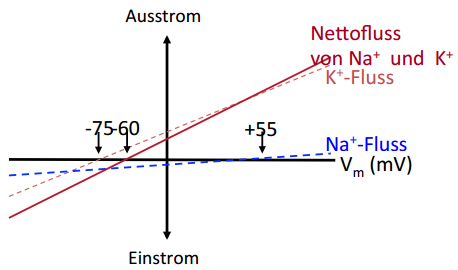
\includegraphics[width=\textwidth]{equilibrium_nernst_01.png}
	\end{subfigure}%
	~
	\begin{subfigure}[b]{0.3\textwidth}
		\centering
		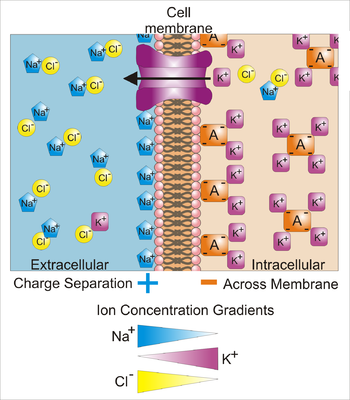
\includegraphics[width=\textwidth]{membrane_potential.png}
	\end{subfigure}
\end{figure}

\subsection{Goldmann-Equation}
\begin{itemize}[noitemsep,nolistsep]
	\item Nernst does not consider multiple ions and permeability.
	\item Goldmann describes membrane potential, with multiple ions and permeability.
	\item Assumes ion flux obeys Nernst/Planck equation.
	\item Assumes ions move across membrane independently, without interaction.
	\item Equilibrium: $P_K:P_{Na}:P_{Cl}$ is $1:0.04:0.45$.
	\item Action potential: $P_K:P_{Na}:P_{Cl}$ is $1:20:0.45$.
	\item $V_m$: Membrane potential.
	\item $P$: Membrane permeability.
	\item $[A^x]$: Ion concentration.
\end{itemize}

\[V_m = \frac{RT}{F} ln(\frac{P_K[K^+]_{out} + P_{Na}[Na^+]_{out} + P_{Cl}[Cl^{-}]_{in}}{P_K[K^+]_{in} + P_{Na}[Na^+]_{in} + P_{Cl}[Cl^{-}]_{out}})\]

\section{Passive (Cable) Membrane Properties}
\subsection{Basic electronics}
\begin{itemize}[noitemsep,nolistsep]
	\item Ohm's Law: $V = I \cdot R$
	\item Kirchoff's Current Law (KCL): The sum of all currents entering and leaving any node in a circuit is zero.
	\item Kirchoff's Voltage Law (KVL): The sum of all voltages around a closed loop is equal to zero.
\end{itemize}

\subsection{Ion channel replacement circuit}
\begin{itemize}[noitemsep,nolistsep]
	\item Ion channel is equal to resistance.
	\item Ion gradient is equal to battery.
	\item Cell membrane is equal to capacitor.
	\item Conductivity $S=\frac{1}{R}$.
	\item Ion resistance is $R = V/I$.
	\item Ion conductivity is $\gamma = g_L = I/V$.
	\item Outward current for an ion is $I_m=g_L(V-E_L)$.
	\item If the concentration of an ion on one side is raised (with a corresponding molecule of opposite charge) and the membrane is permeable for this ion, then the side which has a higher concentration gets more negative, because the ions go to the other side, leaving behind uncompensated negative charges.
\end{itemize}
\begin{figure}[H]
	\centering
	\scalebox{0.7}{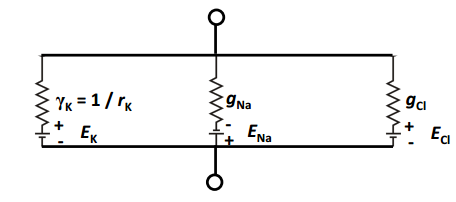
\includegraphics{ion_channel_circuit_01.png}}
\end{figure}
\begin{figure}[H]
	\centering
	\scalebox{0.7}{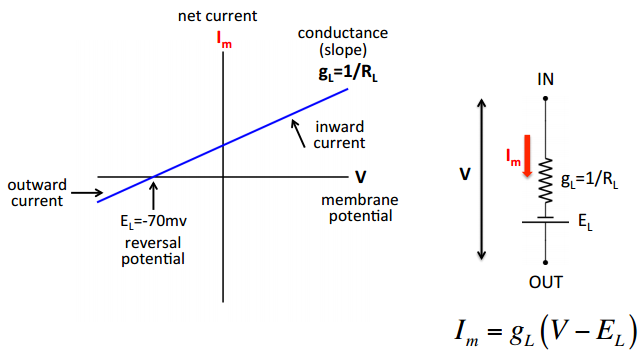
\includegraphics{current_voltage_01.png}}
\end{figure}

\subsection{Single-compartment model}
\subsubsection{Assumptions, configuration}
\begin{itemize}[noitemsep,nolistsep]
	\item Assume isopotential and a sphere of membrane.
	\item $I_e$ is an injected current.
	\item $I_C$ is the capacitive current, discharging the membrane.
	\item There is also a leak current $I_L = g_L(V-E_L)$.
\end{itemize}

\subsubsection{Membrane as electrical circuit}
\begin{itemize}[noitemsep,nolistsep]
	\item $I_e = I_L + I_C$ and $I_L=g_L(V-E_L)$
	\item $C\frac{dV}{dt} = I_C$
	\item $V(t) = V_\infty+(V(0)-V_\infty)e^{-\frac{t}{\tau_m}}$
	\item $V_\infty = E_L + R_LI_e$
	\item Membrane time-constant: $\tau_m = R_LC$
	\item Larger current due to spatial summation.
	\item Less depolarization with small resistance (larger area).
\end{itemize}
\begin{figure}[H]
	\centering
	\begin{subfigure}[b]{0.3\textwidth}
		\centering
		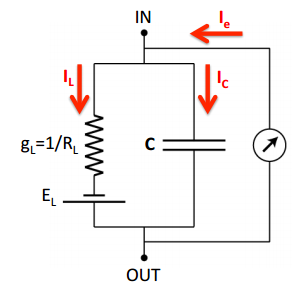
\includegraphics[width=\textwidth]{membrane_circuit_01.png}
	\end{subfigure}%
	~
	\begin{subfigure}[b]{0.5\textwidth}
		\centering
		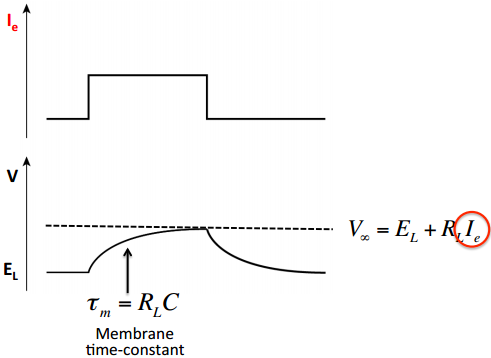
\includegraphics[width=\textwidth]{membrane_circuit_02.png}
	\end{subfigure}
\end{figure}

\subsubsection{Input resistance}
\begin{itemize}[noitemsep,nolistsep]
	\item $A$ is the surface area of the membrane.
	\item $R_L = \frac{r_L}{A}$
\end{itemize}

\subsection{Two ionic currents}
\begin{itemize}[noitemsep,nolistsep]
	\item Equilibrium at $I_L=I_S$
	\item $V_\infty = \frac{g_LE_L+g_SE_S}{g_L+g_S}$
	\item $\tau_m = \frac{C}{g_L+g_S}$
\end{itemize}
\begin{figure}[H]
	\centering
	\begin{subfigure}[b]{0.4\textwidth}
		\centering
		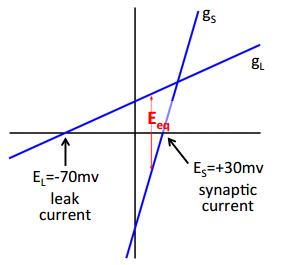
\includegraphics[width=\textwidth]{current_voltage_02.png}
	\end{subfigure}%
	~
	\begin{subfigure}[b]{0.4\textwidth}
		\centering
		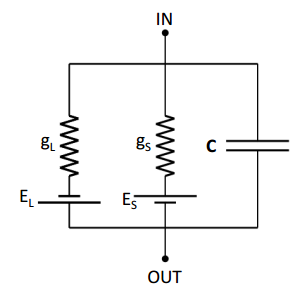
\includegraphics[width=\textwidth]{membrane_circuit_03.png}
	\end{subfigure}
\end{figure}

\subsection{The cable equation}
\[c_m\frac{\partial V}{\partial t} = \frac{1}{2ar_L}\frac{\partial}{\partial x}(a^2\frac{\partial V}{\partial x})-i_m+i_e\]
\begin{figure}[H]
	\centering
	\scalebox{0.7}{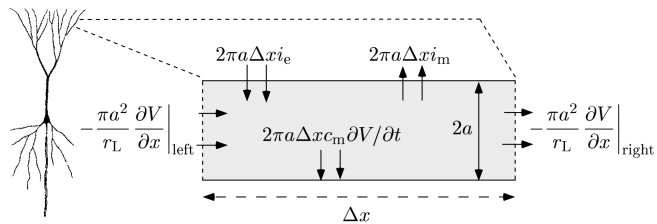
\includegraphics{cable_equation_01.png}}
\end{figure}
\subsubsection{Infinite cable}
\begin{figure}[H]
	\centering
	\scalebox{0.7}{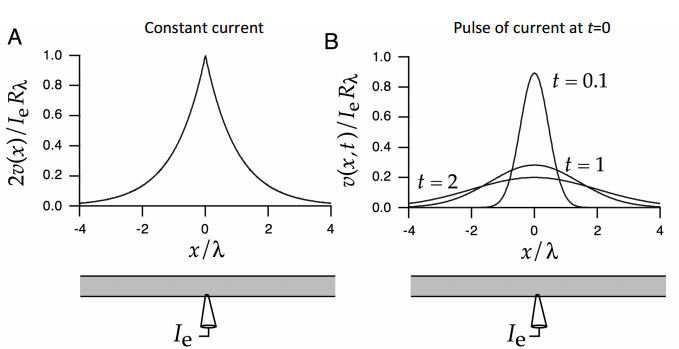
\includegraphics{cable_equation_02.png}}
\end{figure}
\begin{itemize}[noitemsep,nolistsep]
	\item $v(x) = \frac{I_eR_\lambda}{2}\exp(-\frac{|x|}{\lambda})$
	\item $R_\lambda=\frac{r_m}{2\pi a\lambda} = \frac{r_L\lambda}{\pi a^2}$
	\item $\lambda = \sqrt{\frac{ar_m}{2r_L}}$ sets the scale for the spatial variation in the membrane potential.
	\item $\lambda$ is the electronic length, or how far the signal travels.
	\item $\tau_m = r_mc_m$ sets the scale for the temporal variation in the membrane potential.
	\item $v(x,t) = \frac{I_eR_\lambda}{\sqrt{4\pi\lambda^2t/\tau_m}}\exp(-\frac{\tau_mx^2}{4\lambda^2t})\exp(-\frac{t}{\tau_m})$
	\item $a$ is the radius of the axon, about $2\,\mu m$
	\item $r_m$ is the specific membrane resistance, about $1\,M\Omega\cdot mm^2$
	\item $v = V - V_{rest}$
	\item $r_L$ is the longitudinal resistance, about $1\,k\Omega\cdot mm$
	\item $I_e$ is the injected current.
	\item It follows, that increasing $R_m$ also increases $\lambda$. With better isolation, signals travel further.
	\item Increasing the diameter also increases $\lambda$.
\end{itemize}

\subsection{Level of approximation}
\begin{itemize}[noitemsep,nolistsep]
	\item A neuron can be represented by a variable number of discrete compartments.
	\item Compartments represent a region, each with a single membrane potential.
	\item The connections between compartments have resistive couplings.
\end{itemize}

\subsection{Hodgkin-Huxley Equations}
\begin{itemize}[noitemsep,nolistsep]
	\item Model that describes how action potentials in neurons are initiated and propagated.
	\item $n$ and $m$ are probabilities for a gate to be open.
	\item $h$ is the probability that an open channel is not blocked.
	\item The gating variables have a voltage dependence.
	\item $\bar{g}$ values are the maximum conductance possible.
	\item There is no inactivation for potassium, only for sodium.
	\item The membrane does not get locked at positive values.
	\item $\bar{g}_L$ stands for some generic leak.
	\item The functions $n_\infty(V)$, $m_\infty(V)$ and $h_\infty(V)$ determine whether gates serve to activate channels (with depolarization) or inactivate the channel (close with depolarization). $\tau_m$, $\tau_h$ and $\tau_n$ are time constants.
\end{itemize}
\[C\frac{dV}{dt}+\bar{g}_Kn^4(V-V_K)+\bar{g}_{Na}m^3h(V-V_{Na})+\bar{g}_L(V-V_L)+I_{inj}=0\]

\begin{figure}[H]
	\centering
	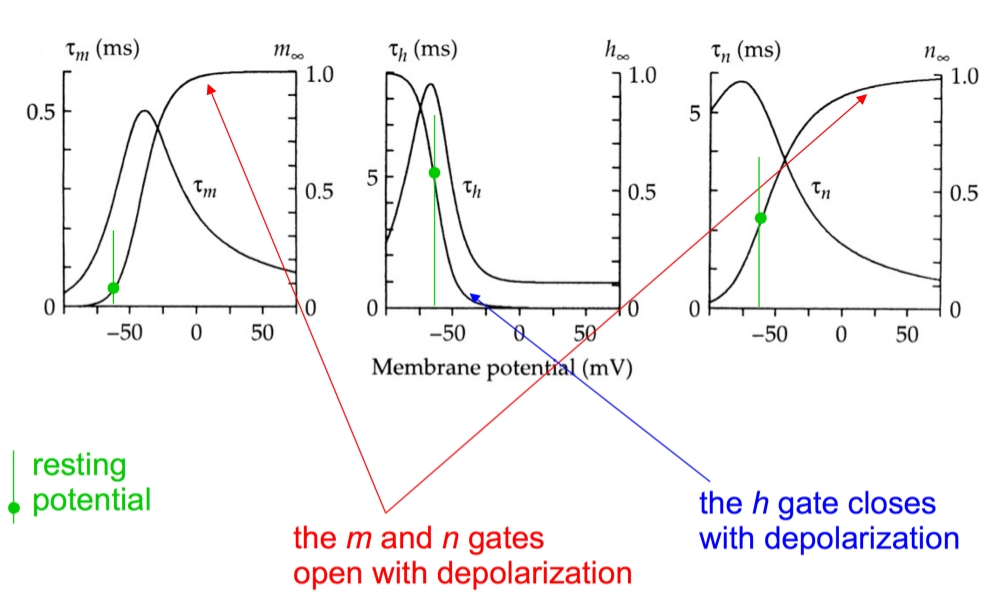
\includegraphics[scale=0.5]{5_8.jpg}
\end{figure} 
\begin{figure}[H]
	\centering
	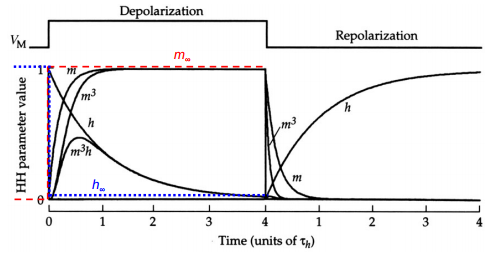
\includegraphics[scale=1.0]{depolarization_01.png}
\end{figure} 

\section{Action Potential}
\begin{itemize}[noitemsep,nolistsep]
	\item Refraction period ensures maximum frequency.
	\item Action potential is about $1$ to $10\,m/s$ fast.
	\item It would take 100 years to go through all axons of the human brain in a serial fashion.
\end{itemize}
\subsection{Equilibrium voltage}
\begin{itemize}[noitemsep,nolistsep]
	\item When $I_m = 0$ and $\frac{dv}{dt}=0$ then
	\item $V=\frac{g_KE_K+g_{Na}E_{Na}+g_{Cl}E_{Cl}}{g_K+g_{Na}+g_{Cl}}$
	\item $I_m = I_{cap}+I_K+I_{Na}+I_{L}$
\end{itemize}

\subsection{Voltage clamp experiment}
\begin{itemize}[noitemsep,nolistsep]
	\item Command voltage is set by the experimenter, the feedback circuit holds the voltage constant.
	\item The voltage clamp allows the membrane voltage to be manipulated independently of ionic currents, allowing the current-voltage relationships of membrane channels to be studied.
	\item With negative feedback circuit, the $Na^+$ current is auto-catalytic. An increase in the voltage increases conductance, which increases the $Na^+$ current, which increases the voltage again.
	\item Voltage and time dependent conductances for $g_{Na}, g_{K}$:
	\subitem $g_{Na}$ increases quickly, but then inactivation kicks in and it decreases again.
	\subitem $g_K$ increases more slowly, and only decreases once the voltage has decreased.
	\item The threshold for action potential initiation is where the inward $Na^+$ current exactly balances the outward $K^+$ current.
\end{itemize}

\begin{figure}[H]
	\centering
	\begin{subfigure}[b]{0.5\textwidth}
    	\centering
		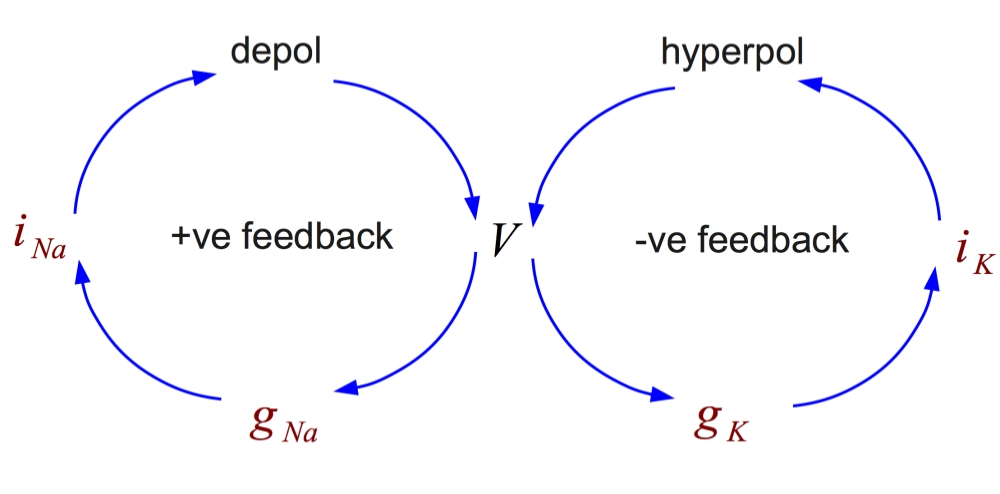
\includegraphics[width=\textwidth]{5_7.jpg}
	\end{subfigure}%
	~
	\begin{subfigure}[b]{0.5\textwidth}
		\centering
		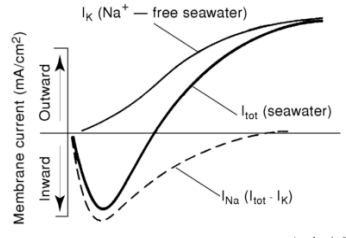
\includegraphics[width=\textwidth]{voltage_clamp_01.png}
	\end{subfigure}
\end{figure}

\begin{figure}[H]
	\centering
	\begin{subfigure}[b]{0.65\textwidth}
    	\centering
		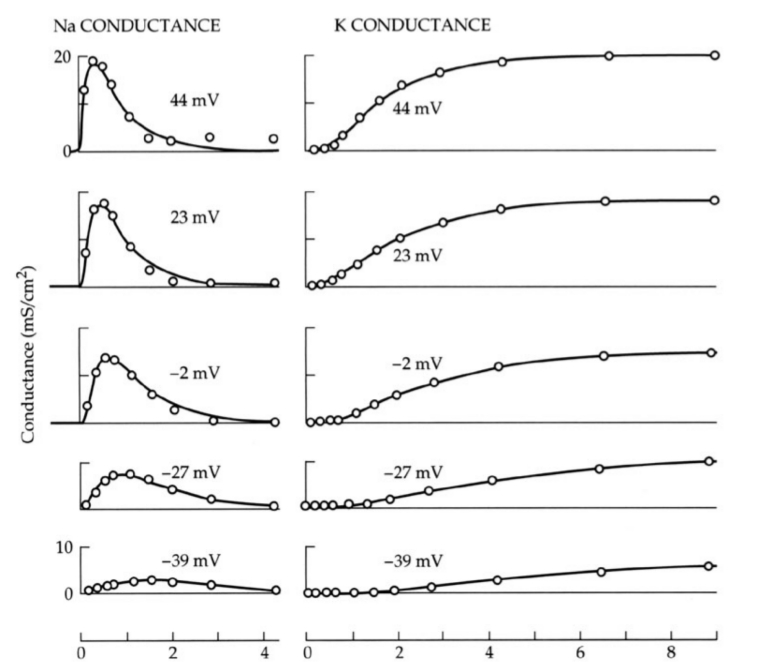
\includegraphics[width=\textwidth]{5_4.jpg}
	\end{subfigure}%
	~
	\begin{subfigure}[b]{0.35\textwidth}
		\centering
		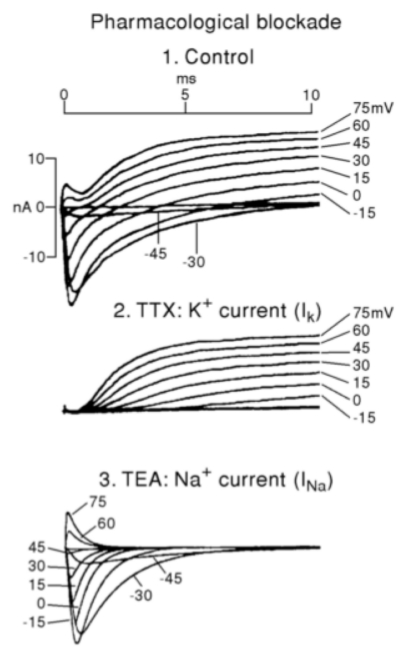
\includegraphics[width=\textwidth]{5_4_2.jpg}
	\end{subfigure}
\end{figure}

\section{Synapse}
\subsection{Introduction}
\begin{itemize}[noitemsep,nolistsep]
	\item First mentioned by Sherrington (1873).
	\item Otto Loewi experimented with the vagus nerve.
	\subitem Stimulating the vagus nerve slows down the heart beat, has an inhibitory function.
	\subitem Ringers solution is a mixture of chemicals in which the heart can continue beating.
	\subitem When switching the solution with one that has been used with an activated vagus nerve, the heart will slow down.
	\item It was found that the ``Vagusstoff'' is acetylcholine (ACh).
	\item The synapses are receptive for nicotine, muscarine and acetylcholine, because of ACh-receptors. This makes certain substances very addictive.
	\item Residual acetylcholine has to be cleared and removed immediately. This happens with acetylcholine esterase enzymes.
\end{itemize}

\subsection{Synapse properties}
\begin{itemize}[noitemsep,nolistsep]
	\item Only vesicles which are already on the presynaptic membrane (docked) will be released after the AP, not all of them.
	\item One single synapse produces only a small potential. More are needed for an actual action potential.
	\item Release of neurotransmitters is calcium dependent.
	\item Probabilistic release of neurotransmitter.
	\subitem In the CNS, most of the time only one vesicle is released with probability $0.2$ to $0.4$.
	\subitem An amplitude histogram shows poisson distribution, which gives the probability of firing.
	\subitem The action potential (probability of firing of synapses, probability of postsynaptic receptors to bind neurotransmitter) give the plasticity (overall probability of passing action potential to postsynaptic neuritic changes).
	\item Single activated synapse is usually not enough. EPSP is about $0.1\,mV$.
	\item The current-voltage lines have bio-measured sigmoid-curves, because channels open with a probability.
\end{itemize}

\subsection{Synaptic mechanism}
\begin{enumerate}[noitemsep,nolistsep]
	\item Synthesis: Building blocks of transmitter substance gets to the terminal where neurotransmitter is synthesized and packed into vesicles.
	\item Release: In response to an AP, the transmitter is released, across the membrane, by exocytosis. The presynapse has voltage-gated $Ca^{2+}$ channels, which will cause an inflow and trigger vesicle fusion (exocytosis).
	\item Receptor activation: The transmitter crosses the synaptic cleft and binds to a receptor.
	\item Inactivation: The transmitter is taken back or inactivated in the synaptic cleft.
\end{enumerate}

\subsection{Receptor types}
\begin{tabular}{|l|l|}
	\hline
	\textbf{Ionotropic receptor} & \textbf{Metabotropic receptor}\\\hline
	Binding site + channel combined & Binding site not associated with channel\\\hline
	Second messenger independent & G-protein or second messenger involved\\\hline
	Short latency action & Longer latency\\\hline
	Rapid response (10 to 50 ms) & Slow responses\\\hline
	Postsynaptic, in general & Pre- and postsynaptic\\\hline
\end{tabular}

\subsection{Synapse types}
\begin{tabular}{|l|l|}
	\hline
	\textbf{Electrical synapse} & \textbf{Chemical synapse}\\\hline
	Simple primitive system & Highly developed structure\\\hline
	Often symmetrical, bidirectional & Polarized, structurally and functionally\\\hline
	Gap junction (connexins) & Pre: active zone, post: postsynaptic density\\\hline
	Very fast, no synaptic delay & Slower, synaptic delay (0.5 ms)\\\hline
	$Ca^{2+}$-independent & Transmitter release requires $Ca^{2+}$ influx\\\hline
	Large synapse & Thousands of small synapses\\\hline
	Limited functions, usually excitatory & Versatile: Excitatory and inhibitory\\\hline
	Synchronized activity & Specific: point to point communication\\\hline
\end{tabular}

\subsection{Receptor overview}
\begin{tabular}{|l|l|l|l|l|}
	\hline
	\textbf{Receptor} & \textbf{Transmitter} & \textbf{Ions} & \textbf{Approx. $E_{rev}$} & \textbf{Agonist}\\\hline
	AMPA & glutamate & Na, K, Ca & $+0\,mV$ & AMPA\\\hline
	NMDA & glutamate & Na, K, Ca & $+0\,mV$ & NDMA\\\hline
	mGLU & glutamate & G-coupled & & \\\hline
	$GABA_A$ & gaba & Cl & $-65\,mV$ & muscimol\\\hline
	$GABA_B$ & gaba & K & $-90\,mV$ & \\\hline
\end{tabular}

\begin{figure}[H]
	\centering
	\begin{subfigure}[b]{0.5\textwidth}
    	\centering
		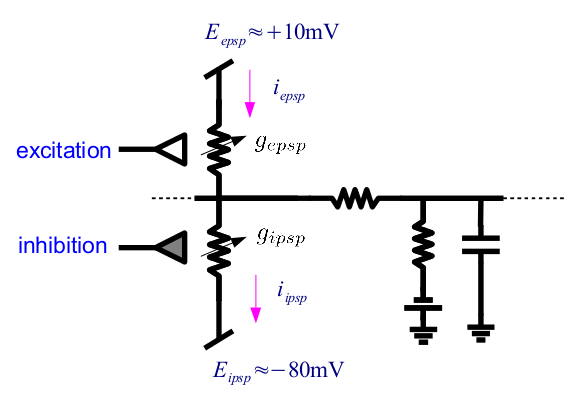
\includegraphics[width=\textwidth]{ex-inhib-elec-membrane.png}
	\end{subfigure}%
	~
	\begin{subfigure}[b]{0.5\textwidth}
		\centering
		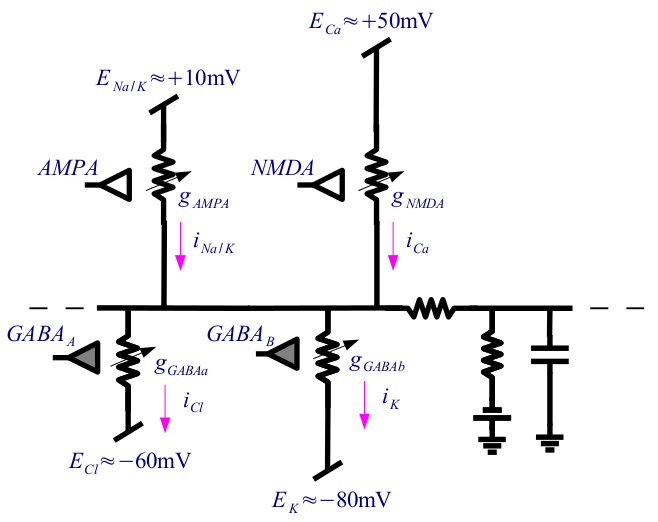
\includegraphics[width=\textwidth]{AMPA-NMDA-GABA-elec-membrane.png}
	\end{subfigure}
\end{figure}

\begin{figure}[H]
	\centering
 	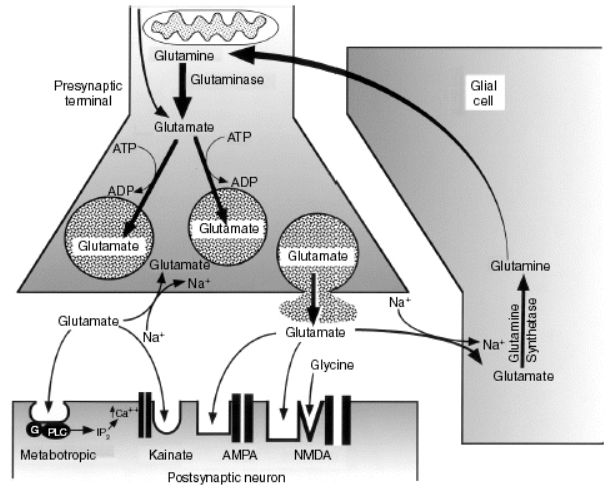
\includegraphics[scale=0.5]{glutamate-neuron.png}
\end{figure} 

\subsection{Glutamate receptors}
\begin{itemize}[noitemsep,nolistsep]
	\item Glutamate enables both synapses, but NMDA is voltage dependent, while AMPA is not.
	\item The receptors end up being conductive for $Na^+$ and $K^+$, as well as $Ca^{2+}$. 10 times more for $Ca^{2+}$ than the others.
	\item $E_S = 0\,mV$
	\item $Ca^{2+}$ inflow causes a calcium cascade: Phosphorylation ($PO_4$) of the channel proteines opens channels even more.
\end{itemize}

\subsubsection{NMDA}
\begin{itemize}[noitemsep,nolistsep]
	\item Voltage dependent.
	\item The channel is blocked by $Mg^+$ below voltages of $-40\,mV$.
	\item The block gets pushed out with more positive voltage.
\end{itemize}

\subsubsection{AMPA}
\begin{itemize}[noitemsep,nolistsep]
	\item Voltage independent.
\end{itemize}

\subsection{GABA}
\begin{itemize}[noitemsep,nolistsep]
	\item GABA-A is for $Cl^-$, ionotropic (fast), $-65\,mV$
	\item GABA-B is for $K^+$, metabotropic (slow), $-90\,mV$
\end{itemize}

\subsection{Neuromodulators}
\begin{itemize}[noitemsep,nolistsep]
	\item Neurotransmitter that is not reabsorbed by the pre-synaptic neuron or broken down into a metabolite.
	\item These end up a longer time in the cerebrospinal fluid, modulating the activity of several other neurons in the brain.
	\item For example norepinephrine, dopamine, serotonine.
\end{itemize}

\section{Plasticity and Learning}
\subsection{Learning and Memory}
\begin{itemize}[noitemsep,nolistsep]
	\item Learning is the acquisition of new information or knowledge.
	\item Memory is the retention of learned information.
	\item The brain has a more complex configuration than given by genes.
	\item There is lots of room for learning (and also need).
	\item Only brain area responsibility and cortex thickness (6 layers) are genetically fixed. But even that can sometimes change later on.
\end{itemize}

\subsubsection{Types of Memory}
\begin{itemize}[noitemsep,nolistsep]
	\item Declarative memory (facts, events)
	\item Non-declarative memory
	\item Procedural memory (skill, habits)
	\item Emotional responses
\end{itemize}

\subsubsection{Connections to Synapses}
\begin{itemize}[noitemsep,nolistsep]
	\item Neurons communicate via AP and are interconnected via synapses.
	\item Information is represented by distributed activity.
	\item Learning and memory is based on changes in synaptic connections.
	\item Synapses get formated, retracted.
	\item Synapse efficacies/plasticity can change.
\end{itemize}

\subsection{Plasticity}
\begin{itemize}[noitemsep,nolistsep]
	\item Modification of postsynaptic potentials (PSPs) evoked by presynaptic spikes.
	\item A: Postsynaptic response triggered by a weak test pulse.
	\item B: Strong stimulation triggers postsynaptic firing.
	\item C: A later test pulse evokes a larger postsynaptic response than initially.
\end{itemize}

\begin{figure}[H]
	\centering
	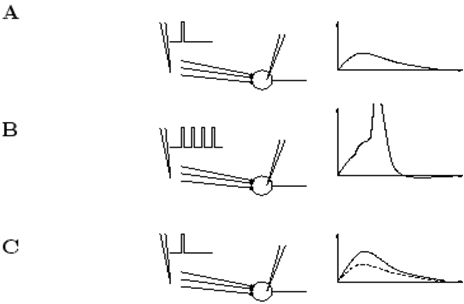
\includegraphics[scale=0.5]{plasticity.png}
\end{figure}

\subsubsection{Parameters that define synapse strengths}
\begin{itemize}[noitemsep,nolistsep]
	\item Neurotransmitter and receptor type
	\item Position of synapse
	\item Availability of vesicles
	\item Re-uptake of transmitters
	\item Neuromodulators, such as dopamine
	\item Postsynaptic cellular processes (such as more or less receptors)
	\item Pre/postsynaptic firing
\end{itemize}

\subsubsection{Models of Synaptic Plasticity}
\begin{itemize}[noitemsep,nolistsep]
	\item There is also non synaptic plasticity, such as dendrite strength, excitability of neurons, isolation of axons.
	\item Phenomenological models show input-output relationships between activity and plasticity.
	\item Biophysical models tell what processes are involved.
	\item Hebb's Postulate: ``When an axon of cell A is near enough to excite cell B or repeatedly or persistently takes part in firing it, some growth process or metabolic change takes place in one or both cells, such that A's efficiency, as one of the cells firing B, is increased''
\end{itemize}

\subsection{Pavlovian Conditioning}
\begin{figure}
	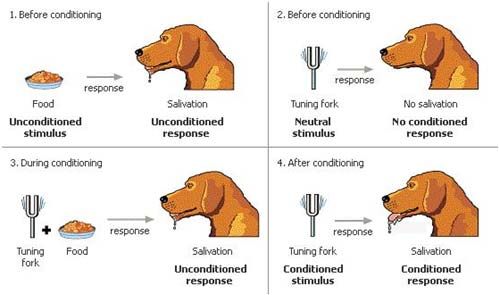
\includegraphics[width=0.9\textwidth]{pavlovian-conditioning.png}
\end{figure}

\subsection{Hebbian Learning}
\begin{itemize}[noitemsep,nolistsep]
	\item Learning based on correlations between pre- and postsynaptic firing.
	\item Uses only variables locally available at the synapse.
	\item Expressed in a rate-based model: $\Delta w_{ij}\propto v_i\cdot v_j$.
	\item Only weight increases, potentiation modeled.
	\item It will lead to instability because of positive feedback loops.
	\item Other rules can be added for weight reduction (depression) and normalization (Oja, BCM).
	\item Hebb's postulate implies constraints for synaptic learning:
	\subitem Direction of information flow (forward).
	\subitem Global effects arise from local learning.
	\subitem Variables are action potentials, synapse weights (efficacy) and neuromodulator/calcium concentration (locally).
\end{itemize}

\subsection{NMDA Synapse}
\begin{figure}[H]
	\centering
	\begin{subfigure}[b]{0.5\textwidth}
    	\centering
		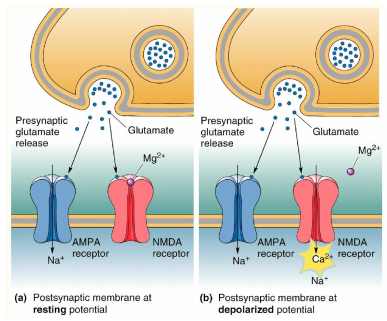
\includegraphics[width=\textwidth]{NMDA_receptor_01.png}
	\end{subfigure}%
	~
	\begin{subfigure}[b]{0.5\textwidth}
		\centering
		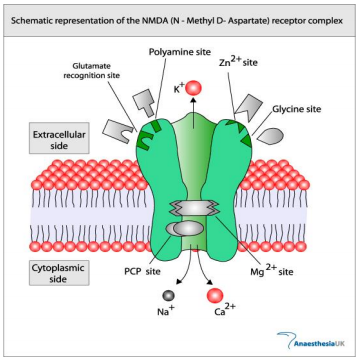
\includegraphics[width=\textwidth]{NMDA_receptor_02.png}
	\end{subfigure}
\end{figure}
\begin{itemize}[noitemsep,nolistsep]
	\item Can act as a coincidence detector for pre- and postsynaptic firing.
	\subitem Backpropagating action potentials.
	\subitem Depolarization from other synapses.
	\item Calcium influx is crucial for plasticity.
	\item Strong NMDA receptor activation gives potentiation.
	\item Weak NMDA receptor activation gives depression.
\end{itemize}
\subsubsection{Potentiation with NMDA}
\begin{itemize}[noitemsep,nolistsep]
	\item Phosphorylation of AMPA receptors makes the synapse stronger.
	\item Synthesis of new AMPA (but not NMDA) receptors.
	\item Transport of AMPA receptors to membrane.
	\item Release probability or quantity of the presynapse can be improved.
\end{itemize}

\subsection{Short-term plasticity (STP)}
\begin{figure}[H]
	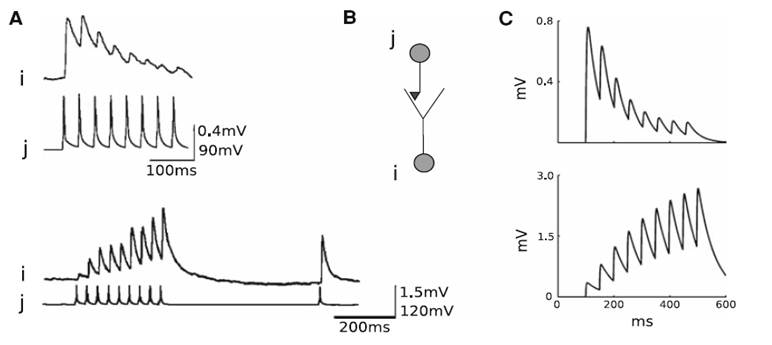
\includegraphics[width=0.8\textwidth]{STP.png}
\end{figure}
\begin{itemize}[noitemsep,nolistsep]
	\item A neuron j fires several times, neuron i fires as well and the spike size is increased(the higher the spike, the more efficient the neuron), but decreases after a short time (caused by loss of vesicles).
	\item Effect goes away in order of milliseconds to seconds.
	\item Short term depression is a safety mechanism.
\end{itemize}

\subsection{Long-term potentiation (LTP)}
\begin{itemize}[noitemsep,nolistsep]
	\item The hippocampus is involved in transferring from short to long term memory.
	\item Tetanus stimulus, strong, high frequent stimulation are required.
	\item A pre- and postsynaptic depolarization at the same time is needed.
	\item Voltage clamp during tetanus prevents LTP from happening.
	\item LTP is cooperative, many weak synapse stimulations give also some effect.
	\item LTP needs a simultaneous depolarization beyond a threshold.
	\item LTP is input specific and can enhance the synaptic effectiveness of a synapse without affecting other synapses in the same cell. This increases the storage capacity of individual neurons.
	\item LTP is associative, weak stimulation in pathways coupled with strong simulation in other pathways can induce LTP.
	\item Stimuli must be delivered at high frequency, because the post-synaptic cell must be depolarized past a certain threshold for LTP.
	\item LTP has a transient early phase ($1-3$ hours), followed by a consolidate later phase ($\geq 24$ hours). The early phase doesn't need new protein synthesis. The later phase needs protein and RNA synthesis for new presynaptic active zones and postsynaptic receptors.
\end{itemize}

\subsection{Long-term depression (LTD)}
\begin{itemize}[noitemsep,nolistsep]
	\item Weakening of the synapse.
\end{itemize}

\subsection{Spike-timing dependent Plasticity (STDP)}
\begin{itemize}[noitemsep,nolistsep]
	\item Not only correlation but also timing of spikes is important.
	\item NMDA receptors and backpropagating action potential creates this timing-dependence of plasticity.
	\item Sign of plasticity is determined by local calcium concentration.
	\item Postsynaptic spike travels back to the dendritic tree and activates voltage-dependent Ca channels.
	\item Presynaptic activity can allow Ca influx through NMDA channels, if the postsynaptic part is sufficiently depolarized.
	\item If pre-spike is soon afterwards followed by post-spike, NMDA-R activity is supralinearly enhanced by depolarization due to backpropagating spike.
\end{itemize}

\begin{figure}[H]
	\centering
	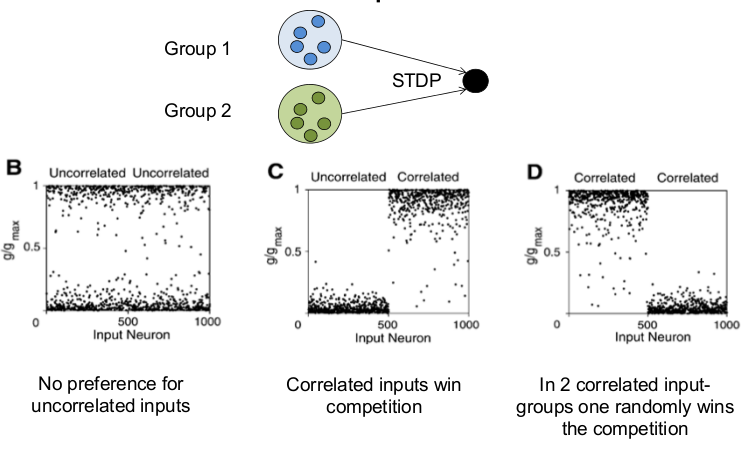
\includegraphics[width=0.8\textwidth]{STDP-consequences.png}
\end{figure}

\begin{figure}[H]
	\centering
	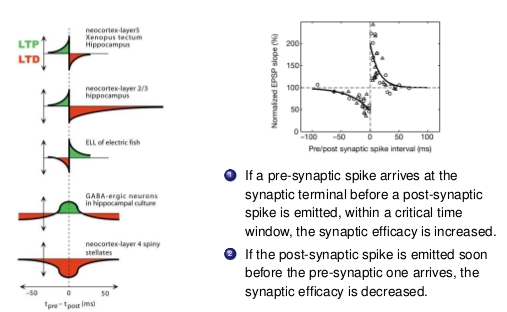
\includegraphics[scale=1]{8_1.jpg}
\end{figure} 

\subsubsection{Functional consequences of STDP}
\begin{itemize}[noitemsep,nolistsep]
	\item Rate normalization, temporal coding, reduced latency, prediction and conditioning.
	\item Only one direction can get stronger, no positive feedback can occur.
	\item STDP can become a simple temporal pattern detector and already fire on the beginning of such a pattern.
	\item Stimulation frequency has an effect on STDP.
	\item Dopamine can extend the LTP timing window or even convert LTD to LTP. Dopamine floats around the cells.
	\item LTP is blocked by AP5. Behavioral success and LTP are correlated.
\end{itemize}

\subsection{Factors that influence plasticity}
\begin{itemize}[noitemsep,nolistsep]
	\item Different plasticity in different brain areas.
	\item Diversity of neuron and synapse types.
	\item Large number of control parameters for plasticity experiments.
	\item Influence of neuromodulators, calcium, drugs, proteins.
	\item Long term vs. short term effects.
	\item Unlikely that a single model explains all plasticity effects found in biology.
\end{itemize}

\section{Rate / Event Coding}
\subsection{Neural Coding}
\begin{itemize}[noitemsep,nolistsep]
	\item Information is encoded by firing of single neurons and firing of populations of neurons.
	\item A neuron encodes information, fires to stimuli.
	\item Firing rate and spike timing encodes information.
	\item Spatial/temporal resolution of different measurement techniques tell us about the neural code.
	\item It is an issue to record from many neurons simultaneously.
	\item There is not much information in the slope of a spike.
\end{itemize}
\begin{figure}[H]
	\centering
	\begin{subfigure}[b]{0.5\textwidth}
		\centering
		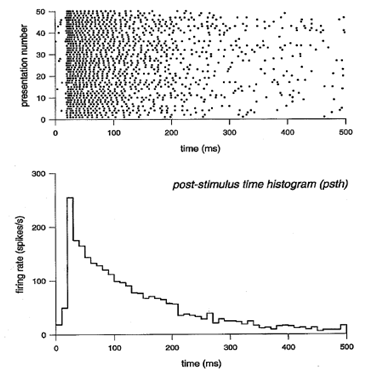
\includegraphics[width=\textwidth]{neural-coding-problem.png}
	\end{subfigure}%
	~
	\begin{subfigure}[b]{0.5\textwidth}
		\centering
		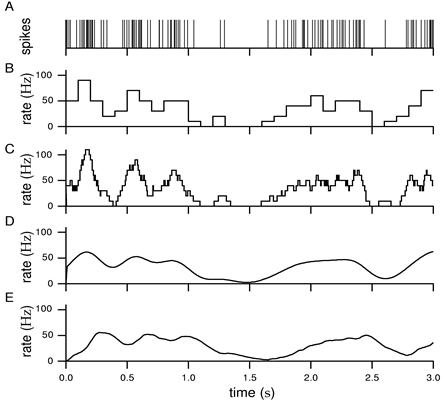
\includegraphics[width=\textwidth]{firing-rate.png}
	\end{subfigure}
\end{figure}
\begin{itemize}[noitemsep,nolistsep]
	\item Raster plot with spikes and histogram. Stimulus takes place at $t = 0$.
	\item Use bins (about 100 ms in time) with a sliding window and a gauss filter and causal filter.
	\item Problematic are intermediate stages, probability of firing, background activity and varying membrane potentials.
	\item Causal filter is $w(\tau) = [\alpha^2\tau\exp(-\alpha\tau)]$
	\item Typically neurons fire between $1\,Hz$ and $200\,Hz$ - often around $40\,Hz$.
\end{itemize}

\subsection{Neuronal Rate Codes}
\begin{itemize}[noitemsep,nolistsep]
	\item Rate = average over time, single neuron, single run.
	\item $v = \frac{n_{sp}}{T}$
	\item Definition of the mean firing rate via a temporal average.
	\item Neuronal gain function (curve). The output spike rate is given as a function of the total somatic input current $I_0$.
	\item Easy to understand, but no timing effects and misleading as more than one stimulus might be encoded.
	\item It takes time to compute a temporal average and behavioral response time is shorter than integration time.
\end{itemize}

\subsection{Peri-Stimulus Time Histogram (PSTH)}
\begin{itemize}[noitemsep,nolistsep]
	\item $\rho = \frac{1}{\Delta t}\frac{1}{K}n_K(t;t+\Delta t)$ where $K$ is the number of trials.
	\item Spike density is an average over several runs of the experiment.
\end{itemize}

\subsection{Tuning Curves}
\begin{itemize}[noitemsep,nolistsep]
	\item Tuning curves show average firing rate response to varying stimulus parameters.
\end{itemize}
\begin{figure}[H]
	\centering
	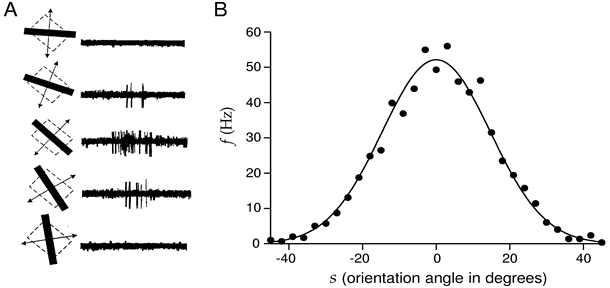
\includegraphics[scale=0.5]{tuning-curve.png}
\end{figure}

\subsection{Orientation Maps}
\begin{itemize}[noitemsep,nolistsep]
	\item Nearby neurons have similar preferred orientations.
	\item Orientation-selective neurons (in the primary visual cortex of cats).
	\item Orientation column and pinwheels.
\end{itemize}

\subsection{Poisson Spike Trains}
\begin{itemize}[noitemsep,nolistsep]
	\item Mathematical model to describe and generate spike trains.
	\item Poission distribution for the number of spikes in interval $T$ with firing rate $r$.
	\item $P_T(n)=\frac{(rT)^n}{n!}\exp(-rT)$
	\item Homogeneous: Constant rate.
	\item Inhomogeneous: Variable rate.
	\item Approximation: Probability of a spike occurring in short interval of length $\Delta t$: $r(t)\cdot\Delta t$
\end{itemize}

\subsection{What a single neuron can encode}
\begin{itemize}[noitemsep,nolistsep]
	\item Places (on entering a particular region).
	\item Grids (regularly arranged triangular grid of locations).
	\item Head-direction, compass-like.
	\item Single cells that respond to only one person.
\end{itemize}

\subsection{Population Rates}
\begin{itemize}[noitemsep,nolistsep]
	\item Rate = average over pool of equivalent neurons (several neurons, single run).
	\item Activity $A=\frac{1}{\Delta t}\frac{n_{act}(t;t+\Delta t)}{N}$
	\item A postsynaptic neuron receives spike input from a population $m$ with activity $A_m$. The population activity is defined as the fraction of neurons that are active in a short interval $[t,t+\Delta t]$ divided by $\Delta t$.
\end{itemize}

\subsection{Population Codes}
\begin{itemize}[noitemsep,nolistsep]
	\item Different cells encode different ranges of the stimulus.
	\item Averaging over a population often meaningless.
	\item Allows accurate reconstruction of the signal, also interpolated between peaks.
	\item Sparse coding: Only few cells are activated.
	\item Retina as an example: Different cells for different light wavelengths.
\end{itemize}

\subsubsection{Population Vector Code}
\begin{itemize}[noitemsep,nolistsep]
	\item Population of neurons with different preferred arm movement directions.
	\item Encoded direction (arrow) corresponds to vectorial addition, weighted by firing rate.
	\item Interesting for brain-computer interfaces.
\end{itemize}

\subsection{Neuronal Event Codes}
\subsubsection{Time-to-first Spike Codes}
\begin{itemize}[noitemsep,nolistsep]
	\item High rate implies fast firing.
	\item Can implement competition among different input cells.
	\item Can be extended to rank-order codes (firing sequence of different neurons).
	\item Is very fast and efficient, has evidence in auditory, visual and somatosensory systems.
	\item Susceptible to noise, requires a reference signal.
\end{itemize}

\subsubsection{Burst- and Temporal Codes}
\begin{itemize}[noitemsep,nolistsep]
	\item Bush-cricket auditory neurons in natural environment.
	\item Preserve very high coding precision in extreme noise.
\end{itemize}
\begin{figure}[H]
	\centering
	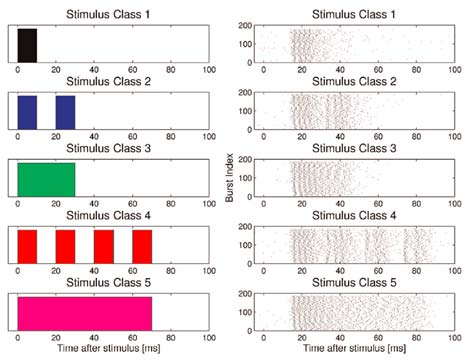
\includegraphics[width=0.6\textwidth]{burst-code.png}
\end{figure}

\subsubsection{Oscillations and Phase Coding}
\begin{itemize}[noitemsep,nolistsep]
	\item Phase: The neurons fire at different phases with respect to the background oscillation.
	\item Phase could code relevant information.
\end{itemize}
\begin{figure}[H]
	\centering
	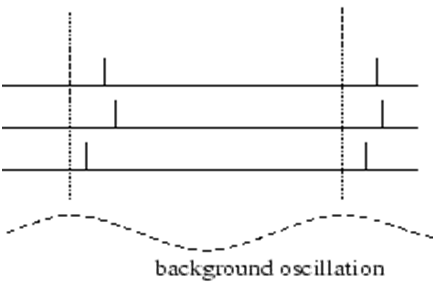
\includegraphics[width=0.4\textwidth]{phase-code.png}
\end{figure}

\subsubsection{Coding by Synchrony}
\begin{itemize}[noitemsep,nolistsep]
	\item Synchrony can encode information.
	\item Neurons can fire (nearly) synchronous.
\end{itemize}

\subsection{Local Field Potential (LFP)}
\begin{itemize}[noitemsep,nolistsep]
	\item Low-pass filtered extracellular recording.
	\item Reflects the integration of membrane currents in a local region.
	\item Dominated by dendritic synaptic activity.
	\item Might encode different properties of the stimulus than single cell firing.
	\item Spike sorting: Assigning spikes to different neurons from extracellular signal (spike shapes are unique for each neuron).
\end{itemize}

\subsection{fMRI}
\begin{itemize}[noitemsep,nolistsep]
	\item Functional magnetoc resonance imaging.
	\item Non-invasive technique for monitoring brain function.
	\item Based on BOLD (blood oxygenation level dependent signal change). Haemodynamic response function (HRF).
	\item Slow temporal resolution.
\end{itemize}

\subsection{Binding Problem}
\begin{itemize}[noitemsep,nolistsep]
	\item Occurs frequently: Visual processing (what, where).
	\item Potential mechanism: Temporal synchrony, hierarchical coding, population coding.
\end{itemize}

\subsection{Averages}
\begin{itemize}[noitemsep,nolistsep]
	\item Spike triggered average: Average over stimulus in short time window before spike.
	\item Sensory neurons typically respond stronger to rapid changes in stimulus properties.
\end{itemize}
\begin{figure}[H]
	\centering
	\begin{subfigure}[b]{0.5\textwidth}
		\centering
		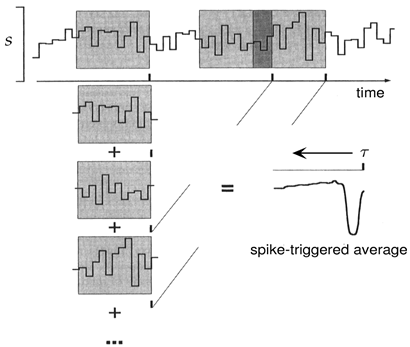
\includegraphics[width=\textwidth]{spike-triggered-average.png}
	\end{subfigure}%
	~
	\begin{subfigure}[b]{0.5\textwidth}
		\centering
		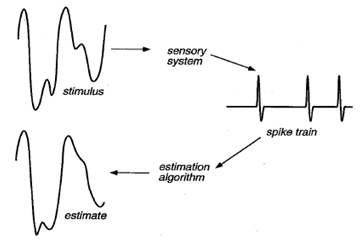
\includegraphics[width=\textwidth]{stimulus-estimation.png}
	\end{subfigure}
\end{figure}

\subsection{Stimulus Reconstruction}
\begin{itemize}[noitemsep,nolistsep]
	\item Allows an observer to reconstruct the stimulus from spike trains.
	\item Probability and information theory is the mathematical background.
	\item Whole stimulus reconstruction may not be relevant.
	\item Evolution may have shaped us to encode particular features better than others, for example faces.
	\item Cells may respond to only particular aspects of stimulus.
	\item Cells may respond to multiple aspects of stimulus.
	\item Artificial stimuli used for studies may be predictable.
\end{itemize}

\section{Perceptron Learning Algorithm}
\begin{figure}[H]
	\centering
	\includegraphics[width=0.3\textwidth]{perceptron.png}
\end{figure}
\begin{itemize}[noitemsep,nolistsep]
	\item Model represents a neuron as a number of inputs $X$ and one Output $Y$. Weights $W$ determine influence of the inputs. $f$ is a function determining the Output, usually $\sum_i(w_i\cdot x_i) \geq \theta$.
	\item Two states: Active or inactive.
	\item Usually bias is added so that $w_0+\sum_i(w_i\cdot x_i)\geq0$ activates the neuron.
	\item This model can create AND/OR/NOT-Gates. Not the XOR/XNOR-Gate however.
\end{itemize}

\subsubsection{XOR impossibility with Perceptrons}
\begin{itemize}[noitemsep,nolistsep]
	\item It is required that $w_0 < 0$, $w_2+w_0 \geq 0$, $w_1+w_0 \geq 0$ and $w_1+w_2+w_0 < 0$.
	\item This causes a contradiction because $2w_0 + w_1 + w_2 < 0$ and $2w_0 + w_1 + w_2 \geq 0$ when adding up the constraints.
	\item XOR is not a linear combination of the inputs.
\end{itemize}

\subsection{Logic gates}
\begin{itemize}[noitemsep,nolistsep]
	\item A table with $N$ inputs has $2^N$ rows. The number of function outputs is then $2^{(2^N)}$.
\end{itemize}
\begin{tabular}{|c|c|c|c|c|c|c|c|c|}
	\hline
	\multicolumn{2}{|c|}{Input} &
	\multicolumn{7}{|c|}{Output}\\\hline
	A & B & AND & OR & NOT & XOR & NAND & NOR & XNOR\\\hline
	  &   & \scalebox{0.4}{\includegraphics{100px-AND_ANSI.png}} & \scalebox{0.4}{\includegraphics{100px-OR_ANSI.png}} &\scalebox{0.4}{\includegraphics{100px-NOT_ANSI.png}} &\scalebox{0.4}{\includegraphics{100px-XOR_ANSI.png}} &\scalebox{0.4}{\includegraphics{100px-NAND_ANSI.png}} &\scalebox{0.4}{\includegraphics{100px-NOR_ANSI.png}} &\scalebox{0.4}{\includegraphics{100px-XNOR_ANSI.png}}\\\hline
	0 & 0 & 0 & 0 & 1 & 0 & 1 & 1 & 1\\\hline
	0 & 1 & 0 & 1 & 1 & 1 & 1 & 0 & 0\\\hline
	1 & 0 & 0 & 1 & 0 & 1 & 1 & 0 & 0\\\hline
	1 & 1 & 1 & 1 & 0 & 0 & 0 & 0 & 1\\\hline
\end{tabular}

\subsection{McCulloch-Pitts Neuron / Perceptron}
\textbf{Similarities to real neurons:}
\begin{itemize}[noitemsep,nolistsep]
	\item Both can be active or inactive.
	\item The input/output is directed.
	\item The activation of a neuron is dependent on a weighted function of other neurons.
\end{itemize}
\textbf{Differences to real neurons:}
\begin{itemize}[noitemsep,nolistsep]
	\item Real neurons exist in continuous time, whereas McCulloch-Pitts neurons operate in discrete time.
	\item Real neurons have degrees of activation, not just on/off.
	\item The activation as a function of the inputs of real neuron is typically not linear or threshold linear.
\end{itemize}

\subsection{Perceptron Learning Algorithm}
\begin{itemize}[noitemsep,nolistsep]
	\item Choose random initial weights.
	\item Calculate output for given input.
	\item If the output is not the expected value, then $e=d-c$, where $d$ is the desired output and $c$ the current output.
	\item Change the weight of inputs and bias by $\Delta w_i=e\cdot\alpha\cdot x_i$. For the bias, always use $x=1$.
\end{itemize}

\section{Hopfield Networks}
\begin{itemize}[noitemsep,nolistsep]
	\item Every node is connected to every other node but not to itself.
	\item Connection weights are symmetric.
	\item $\sum x_iw_i < 0$ is disabled, $\sum x_iw_i \geq 0$ is enabled.
	\item Entire Network is in some state at any time. Set of active units of the entire network is important.
	\item Some states are stable and some are not. While in an unstable state, updating the network leads to a state change.
	\item Stable state is a local minimum. This does however not have to happen.
	\item Bias is an unit that is always on.
	\item Weight of a connection is correlated to frequency of firing together (Hebbian learning).
\end{itemize}

\subsection{Hopfield and Memory}
\begin{itemize}[noitemsep,nolistsep]
	\item A hopfield network is an associative type of memory. Information is stored in the stable states as local minima.
	\item It is important that information is distinct.
	\item Associative memory has room for error but is still recognizable. Convergence to nearby stable states.
	\item Only helpful if reliable input.
	\item If some units are retrievable and all others are set randomly, the correct units will eventually set wrong units right.
\end{itemize}

\subsection{Updates and State Dynamics}
\begin{itemize}[noitemsep,nolistsep]
	\item Nodes can be updated synchronously or asynchronously.
	\item State: Set of units that are active.
	\item Dynamics: Units update their activity level.
	\item When a node is updated, weights are considered from all other active nodes, like with a perceptron.
	\item Asynchronous updates (greedy algorithm) converge to a stable state (sequential), but the converged state can depend on update order.
	\item Asynchronous is either in max-clique state if activity is in $\{0,1\}$ or min-cut if activities are in $\{-1,1\}$.
	\item Synchronous, parallel updates either also go to a stable state, just like asynchronous, or can get stuck in a pair of patterns (flipping or cyclic).
\end{itemize}
\begin{figure}[H]
	\centering
	\includegraphics[width=0.3\textwidth]{hopfield-network.png}
\end{figure}

\section{Feed-Forward Networks}
\begin{itemize}[noitemsep,nolistsep]
	\item Multiple layers of neurons with a certain number of inputs and outputs.
	\item Every laxer of nodes feeds the next layer with inputs.
	\item There is an input and an output layer with hidden layers in between.
\end{itemize}
\begin{figure}[H]
	\includegraphics[width=0.25\textwidth]{Feed_forward_neural_net.png}
\end{figure}

\subsection{Backpropagation and Error function}
\begin{itemize}[noitemsep,nolistsep]
	\item The inputs and desired outputs are given as $S=\{(x,d)^1,\ldots,(x,d)^l\}$.
	\item The error function is given as $E(S) = \sum_i\frac{1}{2}||y(x^i)-d^i||^2$.
	\item The output is a non-linear transformation $y=f(a)$.
	\item $f(a)$ is the activation function, which is usually a sigmoid function.
	\item The error function for a single training sample is $E(S)=\frac{1}{2}(f(x_1w_1+x_2w_2+w_0)-d)^2$.
	\item The output of a simple network is for example $y(x_1,x_2,x_3)=f(x_1w_{21}+f(x_2w_{11}+x_3w_{12}+w_{10})w_{22}+w_{20})$.
	\item $\frac{\partial E(w_1,w_2,w_0)}{\partial w_1}=(f(x_1w_1+x_2w_2+w_0)-d)\cdot f'(x_1w_1+x_2w_2+w_0)\cdot x_1$.
	\item $\frac{\partial E(w_1,w_2,w_0)}{\partial w_2}=(f(x_1w_1+x_2w_2+w_0)-d)\cdot f'(x_1w_1+x_2w_2+w_0)\cdot x_2$.
	\item $\frac{\partial E(w_1,w_2,w_0)}{\partial w_0}=(f(x_1w_1+x_2w_2+w_0)-d)\cdot f'(x_1w_1+x_2w_2+w_0)$.
	\item The error terms travel backwards through the network and get multiplied with the derivative of the activation function of that input. Multiple error terms can just be added up.
	\item The partial derivative of the error $E$ term in relation to the weight $w$ to be adjusted can be added to the weight in order to learn. An additional weighting factor can be added.
\end{itemize}

\section{Signal Propagation in a Network}
\subsection{Avalanche Model}
\begin{itemize}[noitemsep,nolistsep]
	\item For example needed with sensory neurons, as smalls ignals have to be amplified in order to be detectable by the superior areas.
	\item No recurrent connections or risk of positive feedback with risk of explosion.
	\item $(pn)^2$ active neurons per layer. $p$ is a probability and $n$ is the number of neurons that every next layer has more than the previous ones. One neuron from the last layer is connected with $n$ from the next one.
\end{itemize}

\subsection{Synfire Chain}
\begin{itemize}[noitemsep,nolistsep]
	\item The synfire chain is a feedforward structure.
	\item Synchrony is the most important factor for the transmission of the signal.
	\item Noise is important: The chain is usually embedded in a larger network to transmit information. Introducing noise avoids that large-scale synchronization of neuronal firing contaminates the whole network.
\end{itemize}

\subsection{Divergence, convergence}
\begin{itemize}[noitemsep,nolistsep]
	\item A connection is said to be converging if a neuron receives input from several other neurons.
	\item A connection is said to be diverging if a neuron projects to several other neurons.
\end{itemize}

\section{Interacting Neural Populations}
\begin{itemize}[noitemsep,nolistsep]
	\item Neurons can represent information through population codes.
	\item Neurons are tuned to preferred stimuli.
	\item Information is represented by the pattern of activity in a neural population.
	\item Each neuron has a preferred input, for example orientation, that it responds to. The neuron is tuned to that value.
	\item Not every neuron shows clear tuning curves.
	\item Neurons usually do not only respond to their preferred stimulus, but also with decaying strength to close ones.
\end{itemize}

\begin{figure}[H]
	\centering
	\begin{subfigure}[b]{0.3\textwidth}
		\centering
		\includegraphics[width=\textwidth]{one-cell-tuning-curve.png}
		\caption{Tuning curve of one cell}
	\end{subfigure}%
	~
	\begin{subfigure}[b]{0.3\textwidth}
		\centering
		\includegraphics[width=\textwidth]{cell-order.png}
		\caption{Cells ordered by response to $20^\circ$}
	\end{subfigure}
	~ 
	\begin{subfigure}[b]{0.3\textwidth}
		\centering
		\includegraphics[width=\textwidth]{3D-visualisation.png}
		\caption{3D visualization of cell's response to different degrees}
	\end{subfigure}
\end{figure}

\begin{figure}[H]
	\centering
	\begin{subfigure}[b]{0.5\textwidth}
		\centering
		\includegraphics[width=\textwidth]{ape-picture.png}
		\caption{Monkey holding gaze fixed on point $10^\circ$ and light falling in from $20^\circ$}
	\end{subfigure}%
	~
	\begin{subfigure}[b]{0.5\textwidth}
		\centering
		\includegraphics[width=\textwidth]{Retina-Eye-Auditory.png}
		\caption{Visualization of Retina angle ordering cell set R, Eye angle ordering set E,2D result population C and auditory direction set A.}
	\end{subfigure}
\end{figure}

\begin{figure}[H]
	\centering
	\begin{subfigure}[b]{0.3\textwidth}
		\centering
		\includegraphics[width=\textwidth]{Cell-A.png}
		\caption{Cell A $\in$ R}
	\end{subfigure}%
	~
	\begin{subfigure}[b]{0.3\textwidth}
		\centering
		\includegraphics[width=\textwidth]{Cell-B.png}
		\caption{Cell B $\in$ A}
	\end{subfigure}
	~ 
	\begin{subfigure}[b]{0.3\textwidth}
		\centering
		\includegraphics[width=\textwidth]{Cell-C.png}
		\caption{Cell C $\in$ E}
	\end{subfigure}
\end{figure}

\begin{figure}[H]
	\centering
	\begin{subfigure}[b]{0.3\textwidth}
		\centering
		\includegraphics[width=\textwidth]{Cell-D.png}
		\caption{Cell D $\in$ C}
	\end{subfigure}%
	~
	\begin{subfigure}[b]{0.3\textwidth}
		\centering
		\includegraphics[width=\textwidth]{Cell-E.png}
		\caption{Cell E (Not every neuron shows clear tuning curves)}
	\end{subfigure}
\end{figure}

\section{Neuromorphic VLSI}
\subsection{VLSI}
\begin{itemize}[noitemsep,nolistsep]
	\item Very large scale integration technology allows to fabricate chips and memory.
	\item VLSI are usually digital, high power, not fault tolerant or robust, and clocked (synchronous), not massively parallel.
	\item Neuromorphic VLSI contain analog/digital circuits that exploit the physics of silicon to reproduce the bio-physics of neural circuits.
	\item The goals are to understand biological neural systems using standard CMOS VLSI technology as a tool.
	\item Known properties of biological systems can be exploited to design devices for engineering applications.
\end{itemize}

\subsection{Neuron circuits}
\begin{itemize}[noitemsep,nolistsep]
	\item Reproduce physics of neural computation using subthreshold analog circuits and asynchronous digital circuits.
	\item Build autonomous learning behaving systems that can interact with the environment in real-time.
	\item Best exploit for current and future VLSI technologies.
	\item Suited for nano and emerging technologies.
	\item Ideal tools for real- and accelrated-time modeling of neural systems.
	\item Compact, low-power sensory processing devices.
	\item Can interface directly with living systems.
\end{itemize}

\subsection{Circuits}
\subsubsection{n-FET subthreshold}
\begin{itemize}[noitemsep,nolistsep]
	\item $I_0$ current-scaling parameter.
	\item $\kappa_n$ subthreshold slope factor.
	\item $U_T$ the thermal voltage.
	\item $V_g$ the gate voltage, $V_s$ the source voltage, $V_d$ the drain voltage.
	\item The current is defined to be positive if it flows from the drain to the source.
	\item $I_{ds} = I_0e^{\kappa_nV_g/U_T}(e^{-V_s/U_T}-e^{-V_d/U_T})$
	\item If $V_{ds} > 4U_T$ it becomes $I_{ds} = I_0e^{\kappa_nV_g/U_T-V_s/U_T}$
\end{itemize}

\subsubsection{p-FET subthreshold}
\begin{itemize}[noitemsep,nolistsep]
	\item In traditional CMOS circuits, all n-FETs have the common bulk potential $V_b$ connected to ground (GND) and all p-FETs have a common bulk potential connected to the power supply rail ($V_{dd}$).
	\item $I_{ds}=I_0e^{\kappa_p(V_{dd}-V_g)/U_T}(e^{-(V_{dd}-V_s)/U_T}-e^{-(V_{dd}-V_d)/U_T})$
\end{itemize}

\subsubsection{Current Mirror}
\begin{itemize}[noitemsep,nolistsep]
	\item Two MOSFETs of the same size.
	\item $I_{out}=e^{(V_{s1}-V_{s2})/U_T}I_{in}$
\end{itemize}

\subsubsection{Differential-pair}
\begin{itemize}[noitemsep,nolistsep]
	\item $I_b=I_1+I_2=I_0e^{\kappa V_b/U_T}$
	\item $I_1=I_b\frac{e^{\kappa V_1/U_T}}{e^{\kappa V_1/U_T}+e^{\kappa V_2/U_T}}$
	\item $I_2=I_b\frac{e^{\kappa V_2/U_T}}{e^{\kappa V_1/U_T}+e^{\kappa V_2/U_T}}$
\end{itemize}

\subsubsection{Transconductance Amplifier}
\begin{itemize}[noitemsep,nolistsep]
	\item $I_{out}=I_b\tanh(\frac{\kappa}{2U_T}(V_1-V_2))$
\end{itemize}

\subsection{Remarkable circuits}
\begin{itemize}[noitemsep,nolistsep]
	\item McCulloch and Pitts artificial neuron model (first).
	\item Mahowald and Douglas conductance-based silicon neuron, similar to real cortical neurons.
	\item Integrate and fire model (I\&F).
\end{itemize}
\begin{figure}[H]
	\centering
	\begin{subfigure}[b]{0.5\textwidth}
		\centering
		\includegraphics[width=\textwidth]{conductance-based-SI-neuron.png}
		\caption{Conductance-based silicon neuron}
	\end{subfigure}%
	~
	\begin{subfigure}[b]{0.5\textwidth}
		\centering
		\includegraphics[width=\textwidth]{axon-hillock-circuit.png}
		\caption{Axon-Hillock-circuit}
	\end{subfigure}
\end{figure}
\begin{figure}[H]
	\centering
	\begin{subfigure}[b]{0.5\textwidth}
		\centering
		\includegraphics[width=\textwidth]{IanF-circuit.png}
		\caption{Ultra low-power generalized I\&F circuit}
	\end{subfigure}%
	~
	\begin{subfigure}[b]{0.5\textwidth}
		\centering
		\includegraphics[width=\textwidth]{multineuron-circuit.png}
		\caption{Spiking multineuron architectures}
	\end{subfigure}
\end{figure}

\newpage
\subsection{References}
The pictures used in this summary are from the following books and slide sets
and belong to their respective owners. In the context of the summary they are
used for educational purposes only.
\begin{itemize}
\item D. Purves et al.: Neuroscience. Fifth edition. Sinauer
\item Eric Kandel et al.: Principles of Neural Science. Fifth edition.
McGraw-Hill 
\item Peter Dayan, L. F. Abbott: Theoretical Neuroscience, The MIT
Press
\item Christof Koch: Biophysics of Computation. Oxford University Press
\item John Nicholls et al.: From Neuron to Brain. Palgrave Macmillan
\item W. Gerstner et al.: Neuronal Dynamics. From Single Neurons to Networks and
Models of Cognition. Cambridge University Press (2014).
\item Hertz, Krogh, Palmer: Introduction to the Theory of Neural Computation.
Westview Press
\item Bishop: Pattern Recognition and Machine Learning. Springer
\item The lecture slides of the Introduction to Neuroinformatics course of the
years 2012, 2013 and 2014.
\end{itemize}
\end{document}